% !TEX root = thesis-ex.tex
The quark-gluon plasma is a state of matter that comprises of free partons and is formed in extreme conditions of temperature and pressure \cite{SHURYAK198071}.
Its study is motivated by the fact that is the only way to access the dynamics of partons that are otherwise confined within hadrons.
Moreover, its thermodynamic properties are of particular interest since it filled the early universe a few microseconds after the Big Bang \cite{PhysRevLett.34.1353}.
The QGP also forms the core of neutron-stars \cite{Linde_1979} and the recent detection of gravitational waves from a neutron-star merger \cite{PhysRevLett.119.161101} has opened new avenues of investigation \cite{Han:2018mtj, PhysRevD.99.023009, PhysRevLett.122.061101}.
These studies have the potential to provide information into the nuclear equation of state since the dynamics of the merger are sensitive to the behavior of extremely dense nuclear matter \cite{PhysRevD.86.063001}.
The increase in temperatures and density during the merger results in different pre- and post-merger signals of gravitational-waves that suggest a signature of a first-order hadron-quark phase transition at extreme densities \cite{PhysRevLett.122.061102}.
Colliders like RHIC and the LHC on the other hand probe regions that have comparitively low baryon densities.
Lattice QCD calculations in these regions show that the transition between a hadronic gas and the QGP occurs at a temperature of approximately 160 MeV and corresponds to an energy density of 0.5 GeV/fm$^3$ \cite{Borsanyi:2010bp}.
This is a smooth crossover that spans a 20--30 MeV temperature range, and can be seen in the QCD phase diagram shown in Figure~\ref{fig:qcd_phase}.
This phase diagram shows the transition between free quarks and gluons within the QGP and the confined quarks and gluons within hadrons, as a function of temperature $T$ and baryon chemical potential $\mu$.
% matter and had   at $\mu = 0$ is applicable \cite{Aoki:2006we}.

\begin{figure}[htbp]
\begin{center}
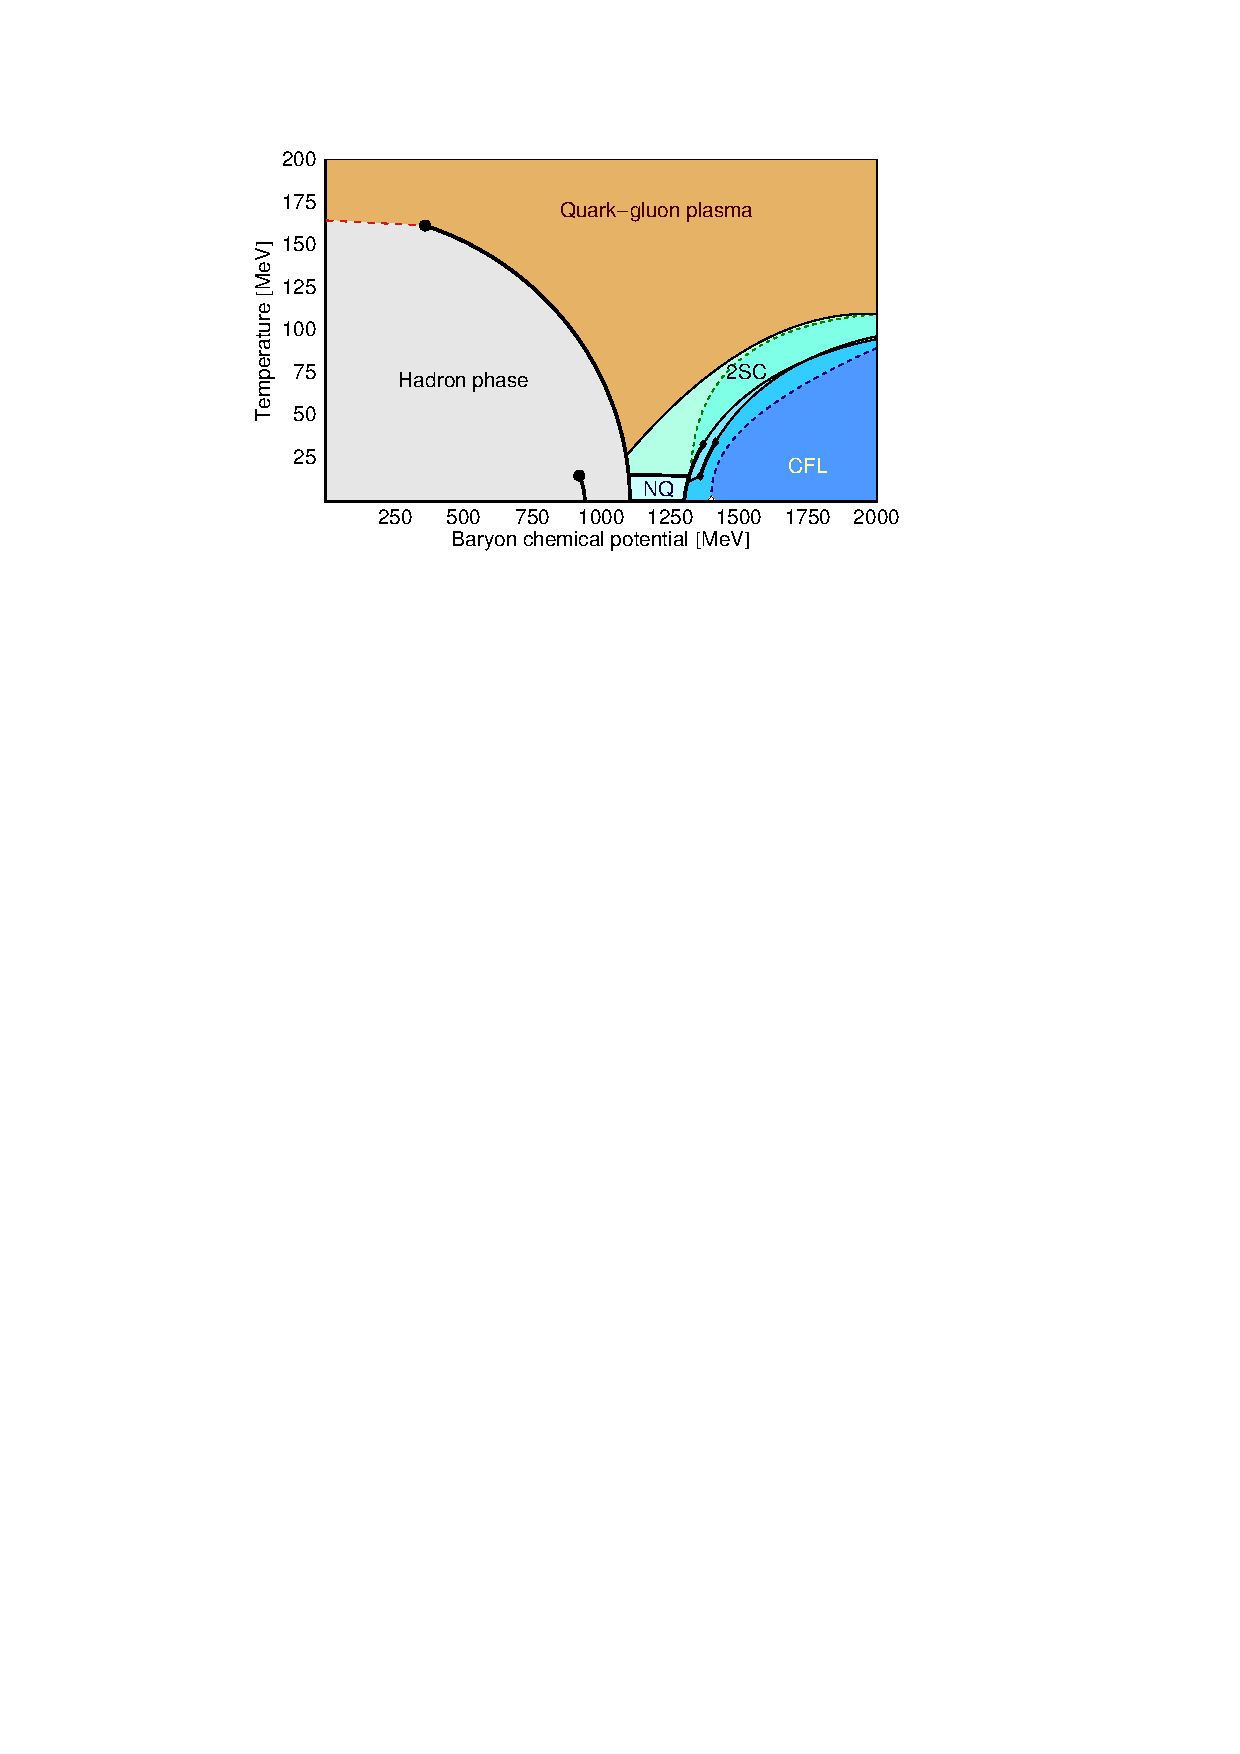
\includegraphics[width=0.45\textwidth]{figures/theory/qcd_phase}
\caption{The QCD phase diagram of nuclear matter as a function of temperature $T$ and baryon chemical potential $\mu$.
The $n\star$ denotes a neutron star.
Figure from from Ref.~\cite{Kronfeld:2012uk}.}
\label{fig:qcd_phase}
\end{center}
\end{figure}

When formed in a heavy ion collision, this state of matter exists for 1-10 fm/c, depending on the collision energy \cite{doi:10.1146/annurev.nucl.46.1.71}.
Thermal photons from the QGP reveal that it reaches temperatures of 300--600 MeV in central collisions at 200 GeV \cite{PhysRevLett.104.132301} and 2.76 TeV \cite{2016235}, showing very little collision energy dependence.
As the QGP cools via expansion, its temperature drops below the critical temperature of QCD phase transitions and it forms a hadron gas.
This process, referred to as a chemical freeze-out, occurs at about 160 MeV \cite{Fodor_2004, ADAMS2005102, PhysRevC.93.024917}.
The hadrons formed in this stage continue to interact with each other, but have energies below the threshold for inelastic particle production, resulting mainly in modifications to their momentum spectra.
This continues till the medium cools further and reaches what is called a thermal freeze-out at 100--150 MeV \cite{PhysRevC.69.024904, PhysRevC.72.014908, PhysRevC.75.024910, PhysRevC.88.044910}.

%These measurements paint a picture of the QGP being formed early in the heavy ion collision.It has a non-uniform energy density and temperature determined by the colliding nuclei and collision energy.The QGP then cools and expands as described by relativistic hydrodynamics, and as its temperature falls below 160 MeV, it experiences a crossover phase transition and hadronizes.This system continues to cool and expand, until at 95 GeV there is a thermal freeze-out.

%The QGP can be further characterized by comparing quarkonia production in heavy ion and \pp\ collisions.

%Supposing that the interactions between quarks and gluons are negligible, their energy density can be written in terms of the temperature $T$ and quark chemical potential $\mu$ as:
%
%\begin{align}
%\varepsilon_g &= \frac{16 \pi^2}{30} T^4 \\
%\varepsilon_q+\varepsilon_{\bar{q}} &= 12 \left( \frac{7\pi^2}{120} T^4 + \frac{1}{4}\mu^2 T^2 + \frac{1}{8\pi^2} \mu^4 \right)
%\end{align}
%Then, the thermodynamical quantities of pressure $P$, entropy density $s$ and baryon number density $\rho_B$ are given by:
%
%\begin{align}
%P = \frac{1}{3} \varepsilon, \qquad s = \left(\frac{\partial P}{\partial T}\right)_\mu, \qquad \rho_B = \frac{1}{3} \left( \frac{\partial P}{\partial \mu} \right)_T
%\end{align}
%
%Using the framework of the MIT Bag Model and assuming the QGP as an ideal gas with a bag constant $\mathcal{B}$ that parameterizes the vacuum pressure \cite{Muller1993, Yagi:2005yb}, the equation of state of the QGP can be written as
%
%\begin{align}
%\varepsilon &= \varepsilon_g(T, \mu) + \varepsilon_q(T, \mu) + \varepsilon_{\qbar} (T, \mu) + \mathcal{B} \\
%P &= P_g(T, \mu) + P_q(T, \mu) + P_{\qbar} (T, \mu) - \mathcal{B}
%\end{align}
%
%This model considers quarks and gluons to move freely inside a ``bag'' and postulates that a deconfined medium can be formed by compressing the bags together.Assuming a baryon free case with $\mu = 0$ and idealizing hadronic matter as a gas of non-interacting massless pions:
%
%\begin{align}
%\varepsilon_\pi = \frac{3\pi^2}{30} T^4, \qquad P_\pi = \frac{1}{3} \varepsilon_\pi
%\end{align}
%%%%%%%%%%%%%%%%%%%%%%%%%%%%

The QGP was initially thought to be a weakly coupled parton gas because of asymptotic freedom from QCD.
The highly energetic collisions such as those at the LHC would imply weak interactions between the partons that make up the plasma \cite{PhysRevLett.34.1353, heinz2013collective, 10.1007/978-1-4020-2705-5_14}.
This would result in rare scatterings between the constituents of the gas, washing out any spatial anisotropies based on ``'lumpy''-ness of the colliding nuclei or the collision geometry.
On the other hand, a strong coupling within the QGP would result in the pressure gradients in the medium being driven by hydrodynamics and spatial anisotropies would be transformed to momentum anisotropies in the particles produced as shown in Figure~\ref{fig:overlap} \cite{Busza:2018rrf}.
In this picture, the non-uniform structure of the colliding nuclei would cause a momentum anisotropy \cite{Ster:1999ib} that would be further enhanced when looking at collisions that are less central and do not have perfect overlap between the colliding nuclei \cite{Poskanzer:1999ea, Pinkenburg:1999ya}.
These observations were seen in azimuthal correlation measurements implying that the medium is indeed strongly coupled \cite{Aaboud:2018ves, PhysRevLett.91.182301, Sirunyan:2017fts, PhysRevLett.116.132302}.

\begin{figure}[htbp]
\begin{center}
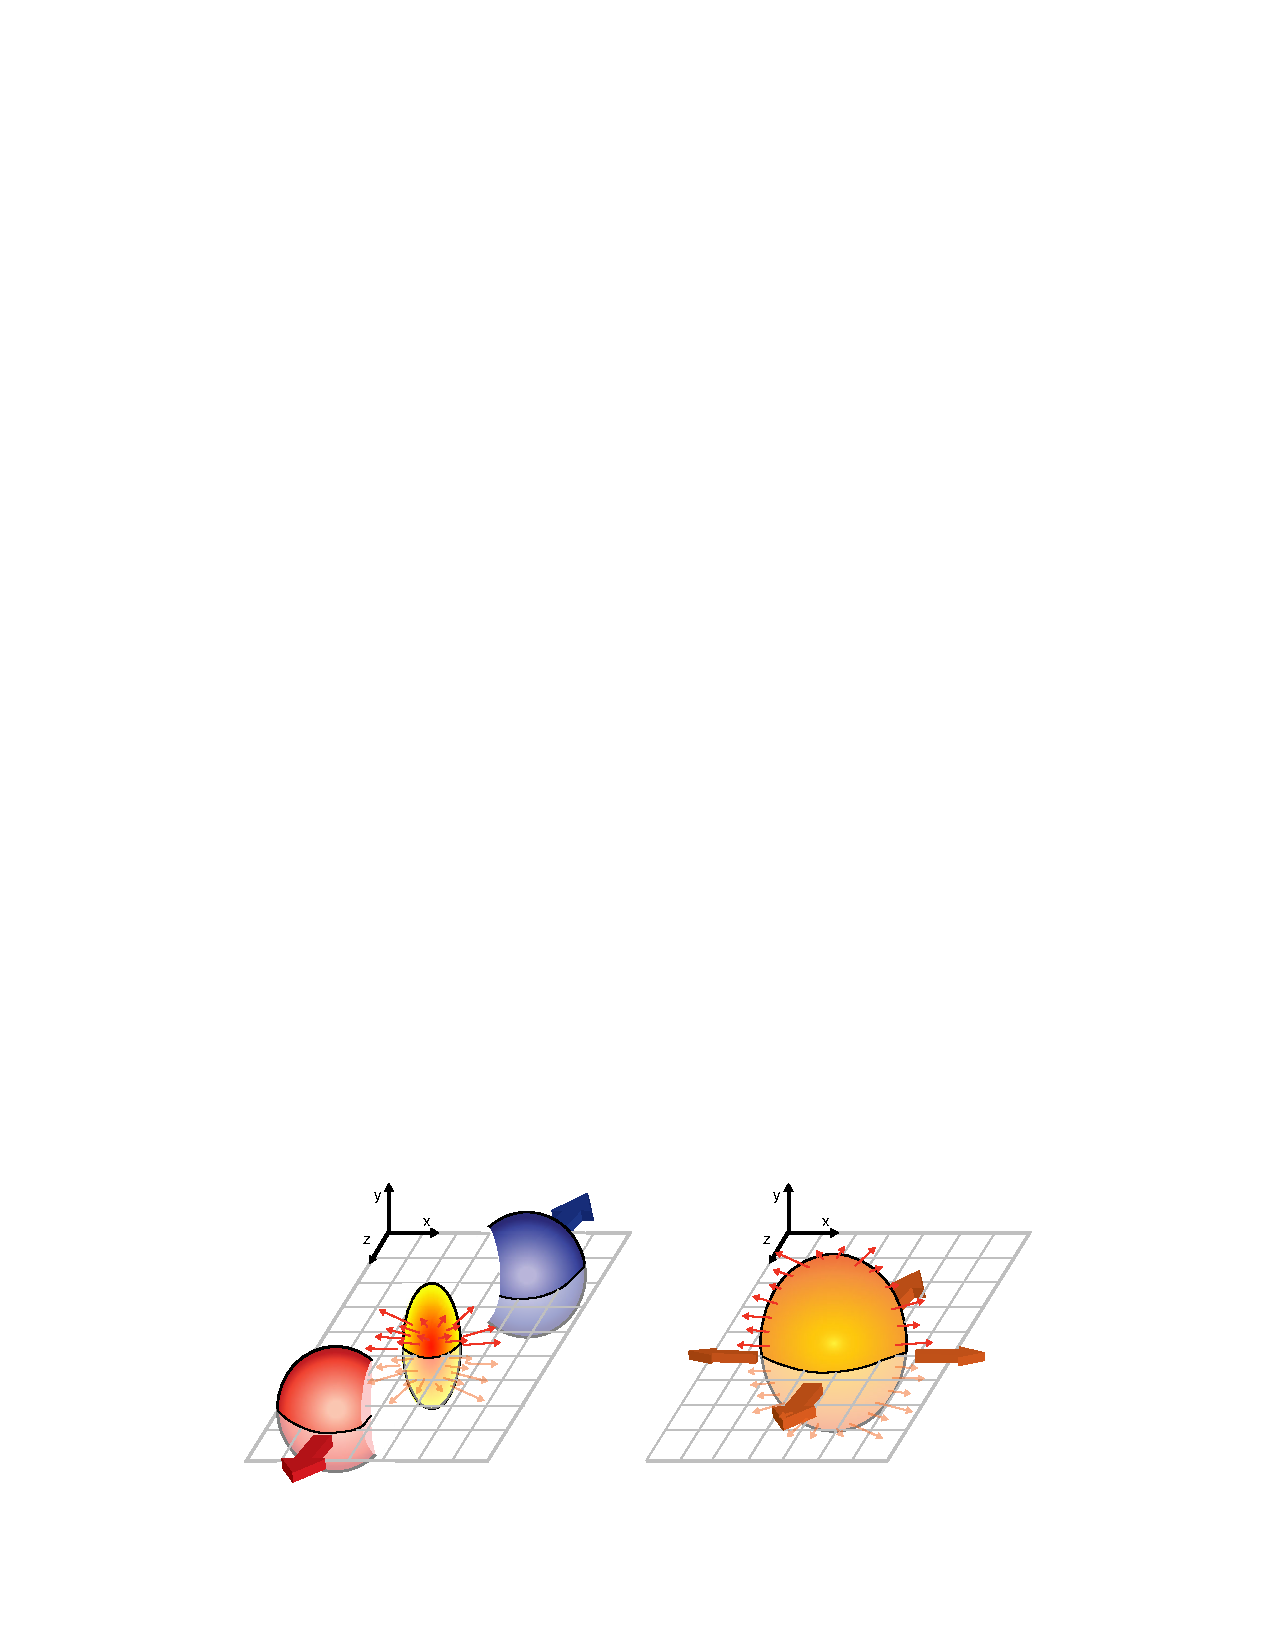
\includegraphics[width=0.85\textwidth]{figures/theory/overlap}
\caption{Schematic diagrams of the initial overlap region (left) and the final spatial anisotropy generated (right).
Taken from \cite{RevModPhys.90.025005}.}
\label{fig:overlap}
\end{center}
\end{figure}


%At the peak energy density of the collision, the system cannot be described at the level of hadrons, and has to be described in terms of quarks and gluons.The initial anisotropic energy density being reflected in the azimuthal variation of particle production implies a strongly coupled medium that expands hydrodynamically, with a faster expansion in the direction of larger gradients and hence resulting a momentum anisotropy.
%A Fourier Transform of the angular distribution of charged hadrons in the collision debris can quantify these momentum anisotropies and give the anisotropic flow coefficients $v_n$, defined as :

The azimuthal angular distribution of particles produced in a heavy ion collision can be expanded in a Fourier series as \cite{Poskanzer:1998yz}: 

\begin{align}
\frac{d\bar{N}}{d\phi} = \frac{N}{2\pi} \left( 1 + 2 \sum_{n=1}^{\infty} v_{n} \cos(n(\phi-\Psi_n)) \right).
\end{align}
where  $N$ is the particle yield, $\phi$ is the azimuthal angle in the transverse plane and $\Psi_n$ is the orientation of the $n^{\mathrm{th}}$ order symmetry plane and is called the reaction plane.
The reaction plane, along with the participant plane, are shown in Figure~\ref{fig:reaction_plane}.
The coefficient $v_n = \langle \cos[n(\phi_i - \Psi_n)] \rangle$ is the magnitude of the $n^{\rm{th}}$ order azimuthal anisotropy, and is referred to as the flow harmonic.
The first harmonic $v_1$ is called directed flow because it indicates a particular direction, while the second harmonic $v_2$ is called elliptic flow since the azimuthal distribution in polar coordinates for $v_2 \neq 0$ is an ellipse.
These are shown in Figure~\ref{fig:flow_v1_v2} \cite{Voloshin:2008dg}.
The azimuthal correlations that are a result of flow can be described by relativistic hydrodynamics \cite{Teaney:2001av, HIRANO2006299}.
A comparison of anisotropies measured in terms of $v_n$ in Ref.~\cite{ALICE:2011ab} and a hydrodynamic model described in Ref.~\cite{Niemi:2015qia} is shown in Figure~\ref{fig:flow_coeff}.


\begin{figure}
\begin{center}
  \begin{minipage}[b]{0.4\textwidth}
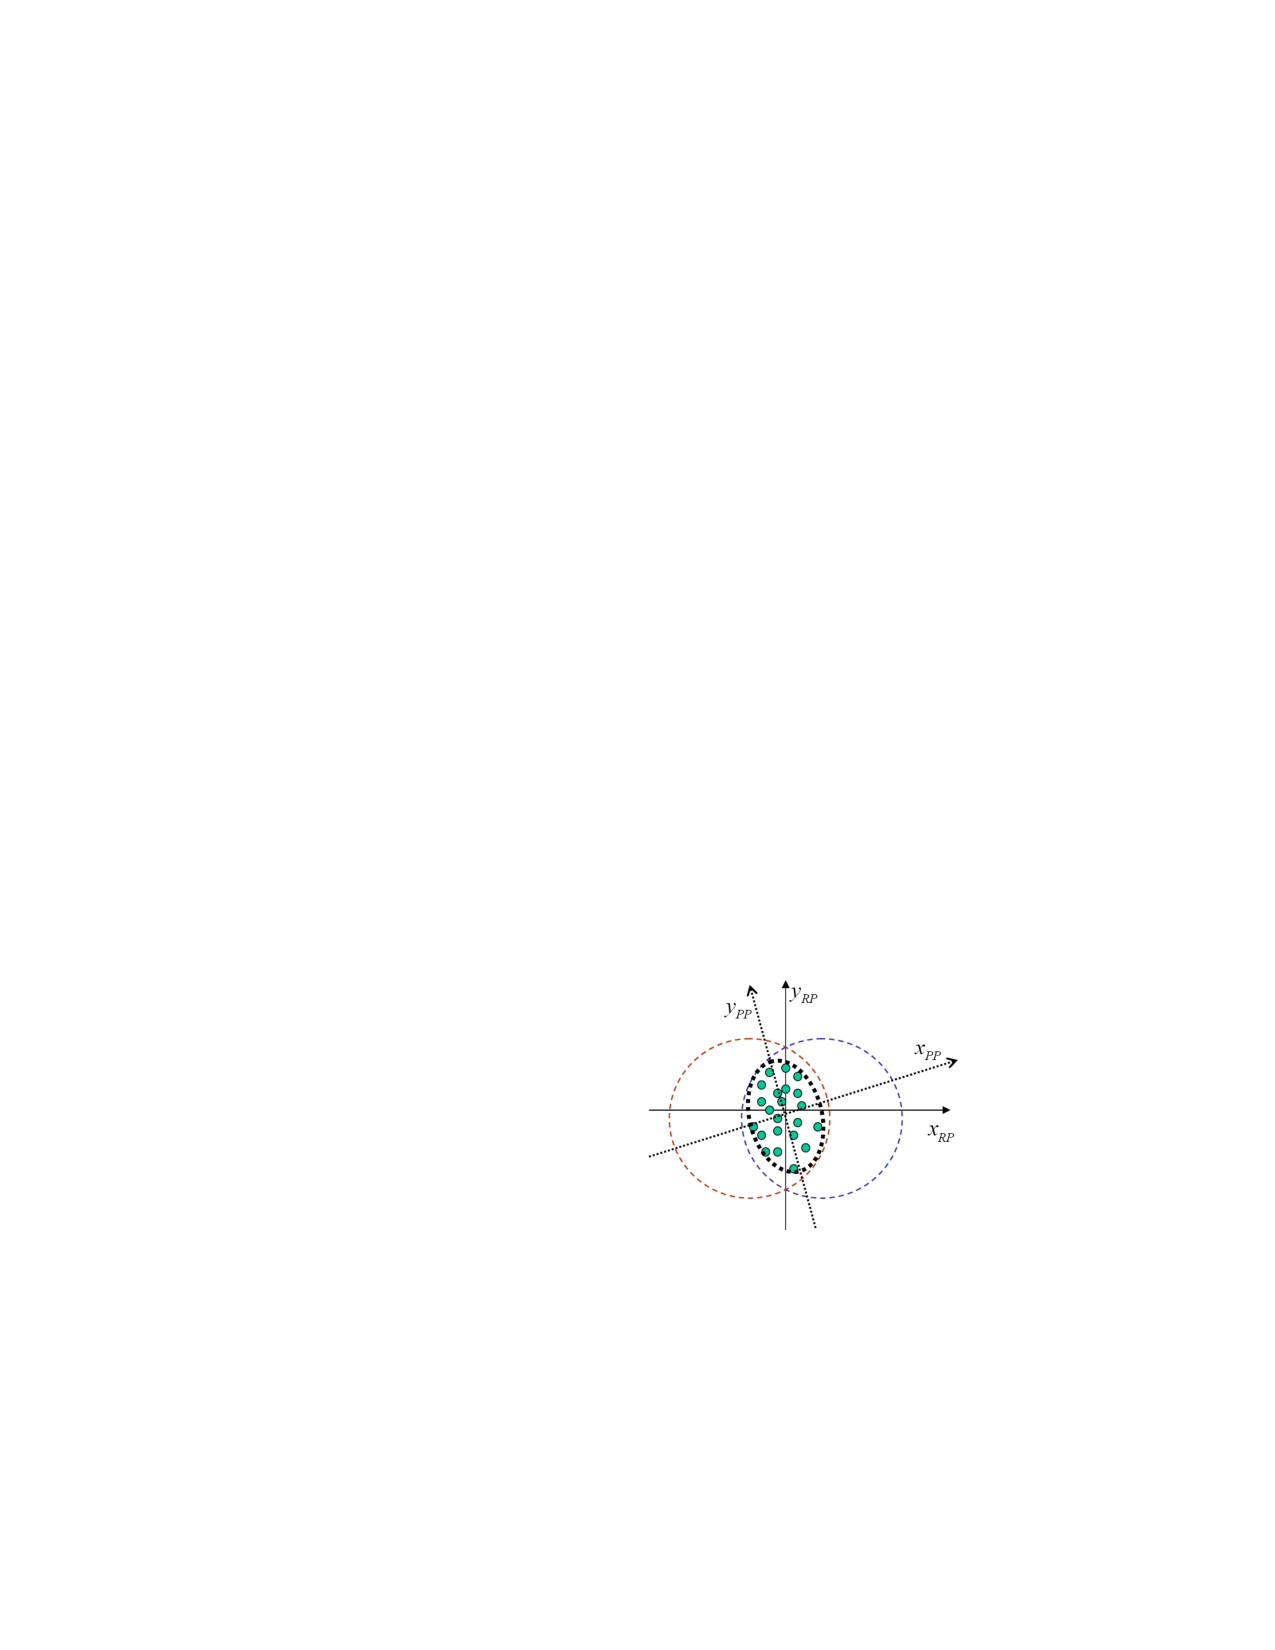
\includegraphics[width=\textwidth]{figures/theory/reaction_plane}
\caption{Definitions of the Reaction and Participant Plan coordinate systems.
Figure taken from Ref.~\cite{Voloshin:2008dg}.}
\label{fig:reaction_plane}
  \end{minipage}
 \qquad  \qquad  \qquad
  \begin{minipage}[b]{0.4\textwidth}
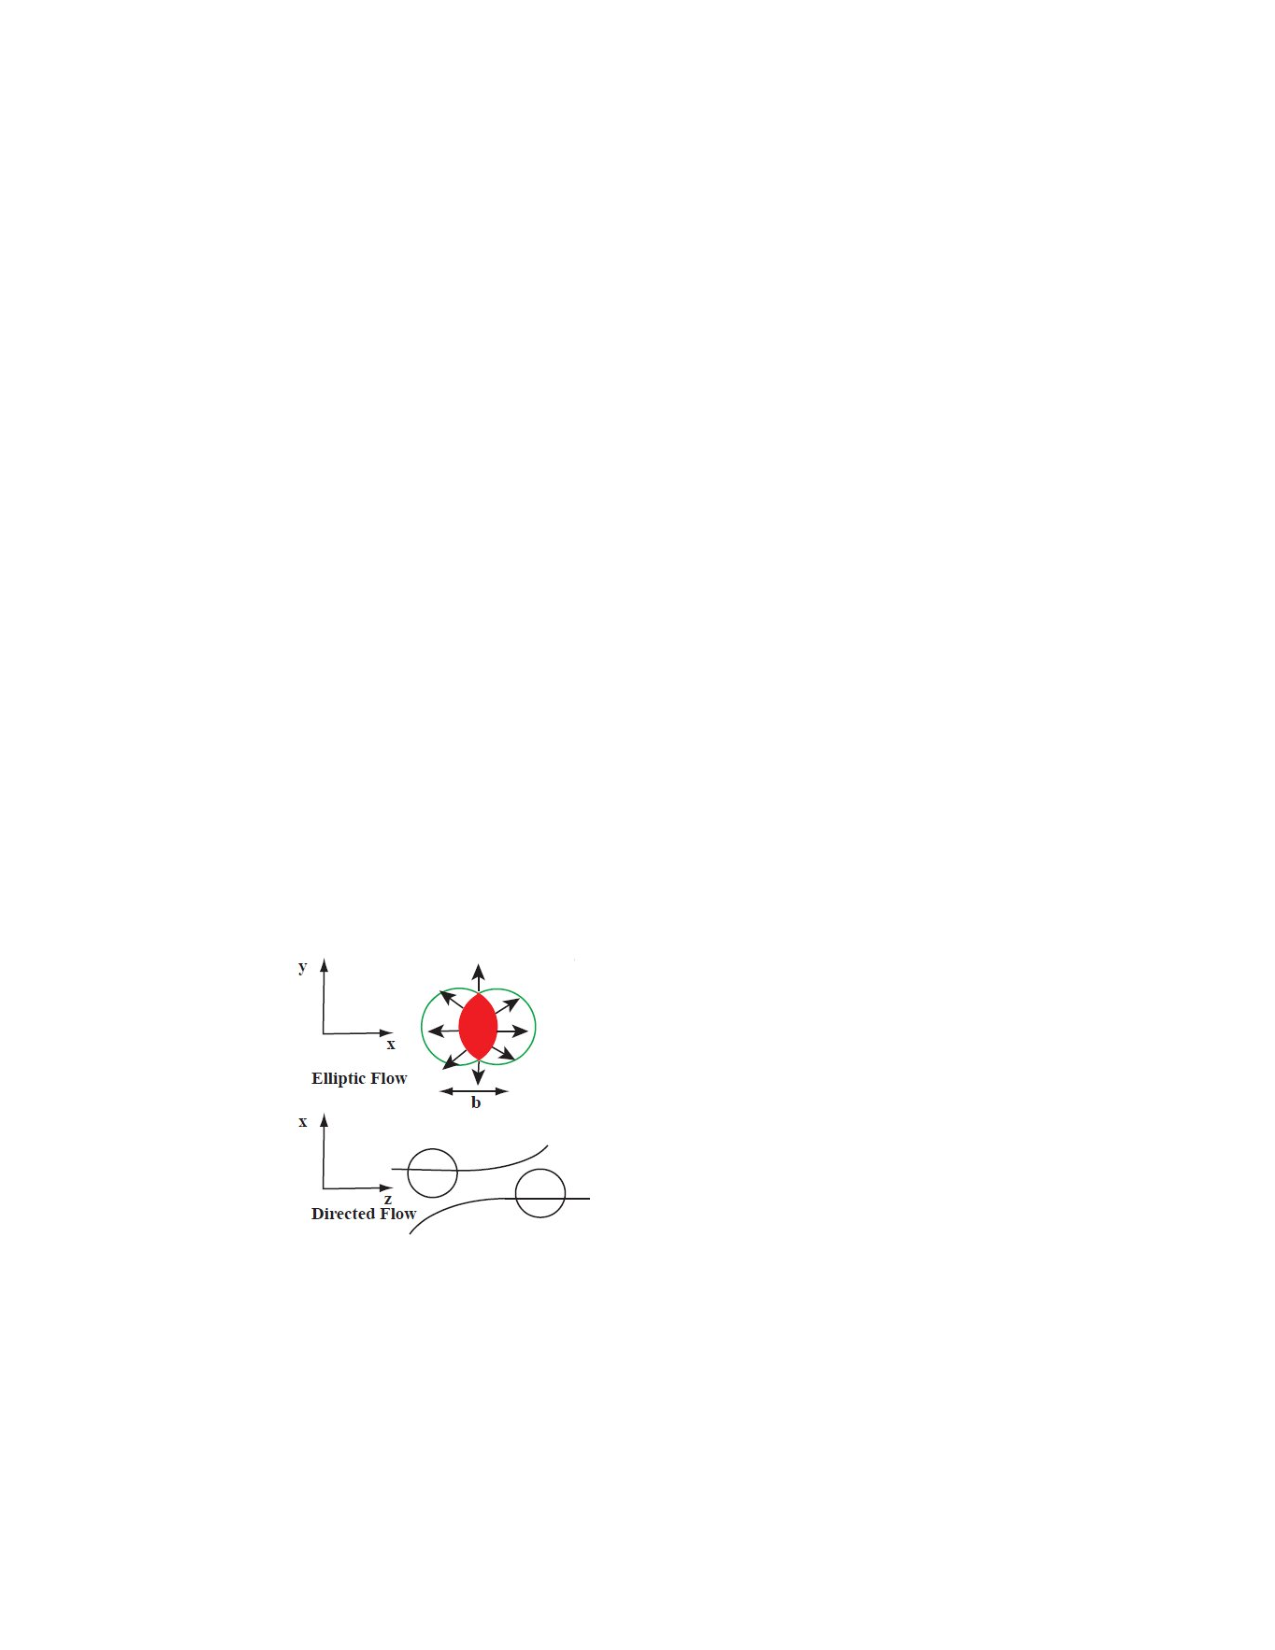
\includegraphics[width=\textwidth]{figures/theory/flow_v1_v2}
\caption{Schematics of elliptic and directed flow.
Figure taken from Ref.~\cite{Voloshin:2008dg}.}
\label{fig:flow_v1_v2}
  \end{minipage}
  \end{center}
\end{figure}

\begin{figure}[htbp]
\begin{center}
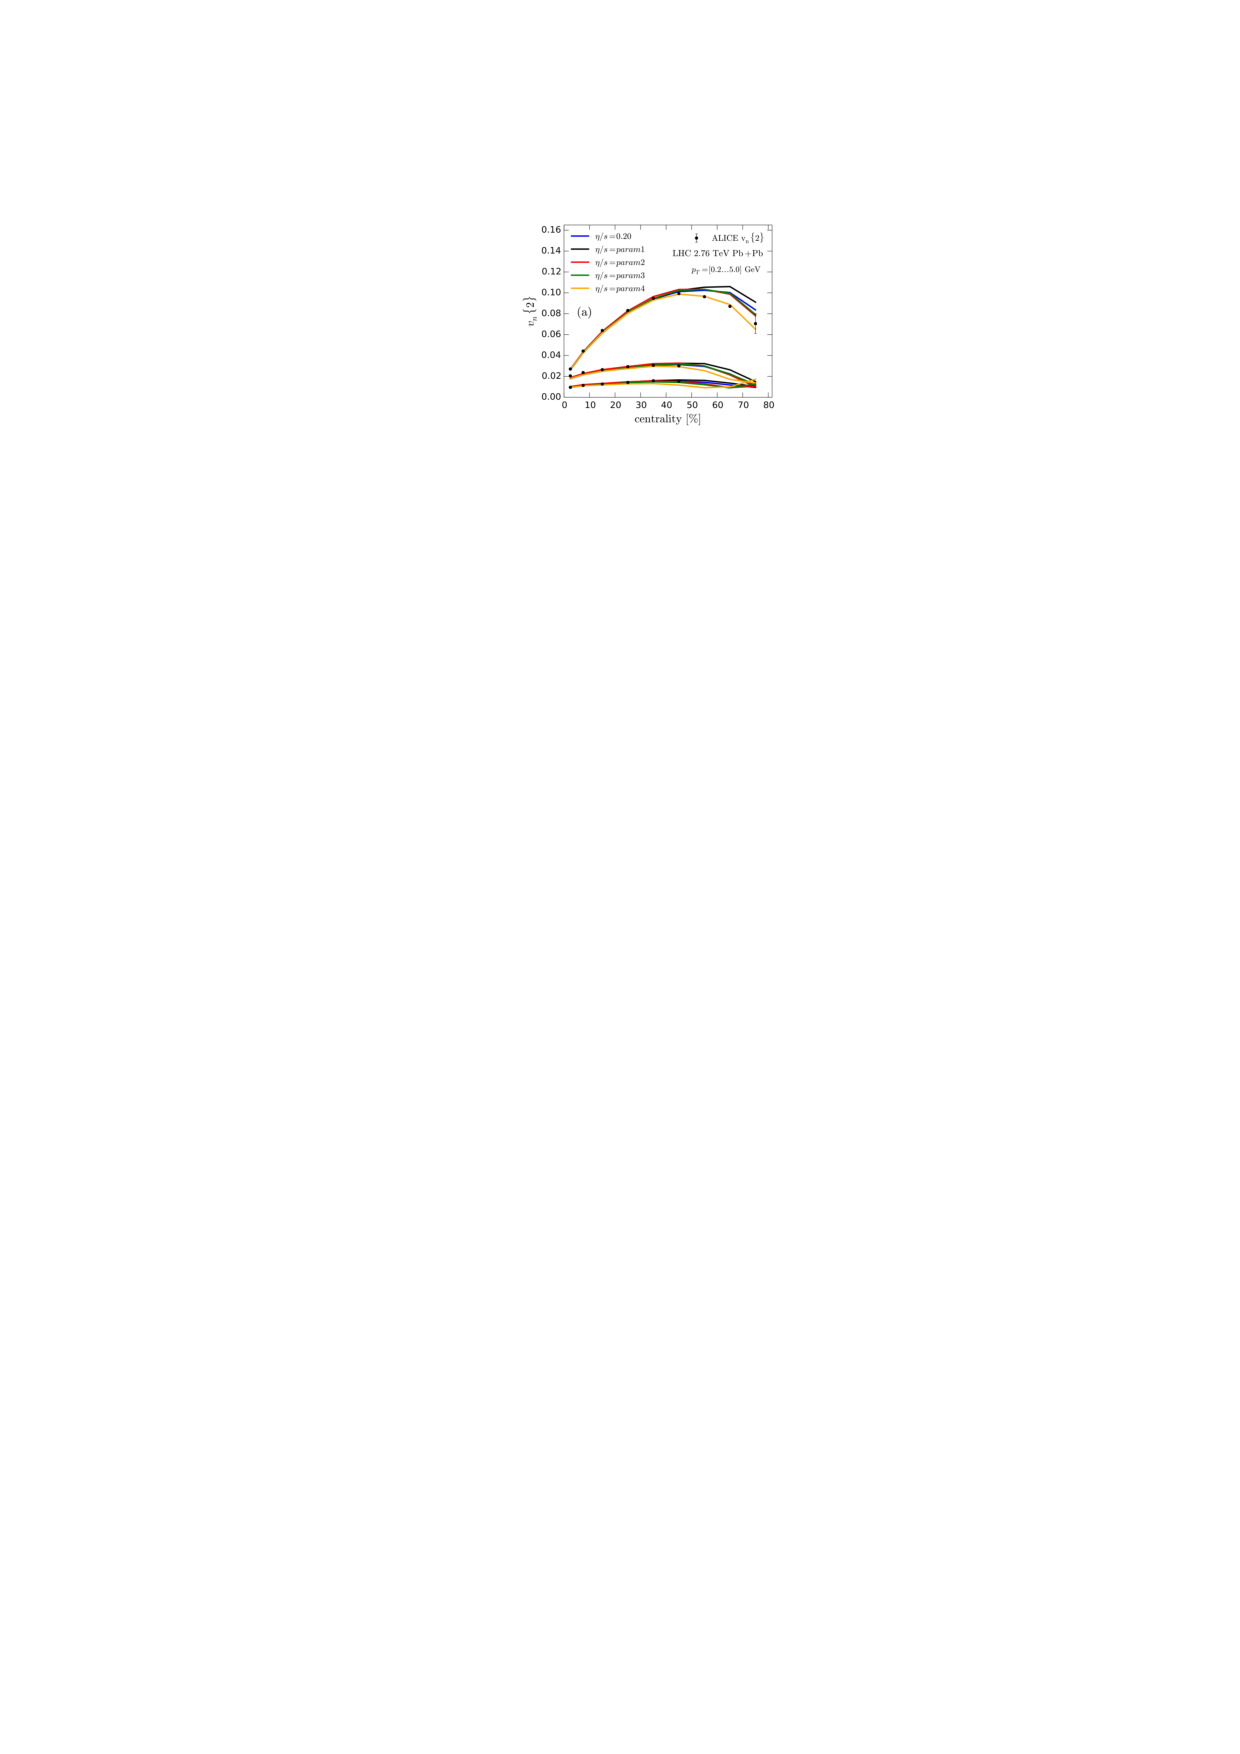
\includegraphics[width=0.45\textwidth]{figures/theory/flow_coefficients}
\caption{Comparison of a hydrodynamic model from \cite{Niemi:2015qia} to anisotropy measurements by ALICE \cite{ALICE:2011ab} for different parameterizations of $\eta / s $ and for different $v_n$, {\it{n}} = 2, 3, 4 from top to bottom, as a function of collision centrality.
Figure taken from Ref.~\cite{Busza:2018rrf}.}
\label{fig:flow_coeff}
\end{center}
\end{figure}

The measured anisotropies can be used to constrain the specific viscosity given by the ratio of viscosity to entropy density, $\eta / s$, and have shown that the QGP is a near perfect liquid with an $\eta / s$ of near the theoretical minimum of $1/4\pi$ \cite{ARSENE20051, GYULASSY200530}.
In fact, this low shear viscosity is what allows the initial fluctuations in the energy density to survive the chemical freeze-out.

























